\documentclass[10pt,a4paper,twocolumn]{article}
\usepackage[utf8]{inputenc}
\usepackage[T1]{fontenc}
\usepackage[margin=1.8cm,columnsep=0.7cm]{geometry}
\usepackage{amsmath,amssymb,bm}
\usepackage{booktabs}
\usepackage{graphicx}
\usepackage{xcolor}
\usepackage{enumitem}
\usepackage{caption}
\usepackage[colorlinks=true,linkcolor=blue!50!black,citecolor=blue!50!black,urlcolor=blue!50!black]{hyperref}
\captionsetup{font=small,labelfont=bf}
\graphicspath{{../../figures/}}
\setlist{nosep,leftmargin=*}
\newcommand{\E}{\mathbb{E}}

\title{\textbf{Learning hierarchical Potts models:\\ factored attention versus masked diffusion on a controlled protein-like benchmark}}
\author{Youssef Kabbaj}
\date{October 2026}

\begin{document}
\twocolumn[
\maketitle
\begin{abstract}
Generative models of protein families are usually judged against finite alignments whose true distribution is
unknown. We build instead a fully controlled benchmark: a tree of Potts models (3 families, 9 subfamilies, 18 clades)
whose parameters differ by a known, decreasing amount at each level, and from which we sample 180\,000 sequences of
length 60. On this ground truth we compare two ways to learn the distribution. The first is a factored-attention
transformer whose output is exactly a Potts model ($J_{ij}=\sum_h\mathrm{softmax}(Q^hK^{h\top})_{ij}V^h$), trained by
pseudo-likelihood, either unconditioned or conditioned on hierarchical tags. The second is a masked (absorbing-state)
diffusion model trained on a bound of the full likelihood. The factored-attention model recovers every true contact
and learns mostly the \emph{ancestral} couplings, but generates the three families in wrong proportions (22/12/66\%).
We trace this to pseudo-likelihood never seeing the partition function: the family weights are the small residual of
a near-cancellation between energy and entropy. Hierarchical tags fix the proportions; the tag-specific information
is then carried mainly by the fields, not the couplings. The diffusion model, without any label, generates families
and clades in the right proportions, reaches pooled correlation fidelity $r_C=0.992$ (fresh true samples: 0.994), and
per clade matches or beats the Potts model that is given the clade tag. Its conditional probabilities are as close
to the truth as those of the tag-conditioned Potts model. The price is interpretability and a 10--100$\times$ higher
training cost.
\end{abstract}
\vspace{1em}]

%=====================================================================
\section{Introduction}
%=====================================================================
Protein families are hierarchical: families split into subfamilies and then into finer clades that share a fold but
differ in residue preferences. A generative model of such data should get every level right. It should reproduce the
statistics of each clade, place generated sequences in the right branch, and generate the branches in the right
proportions. With real alignments none of this can be checked exactly: the true distribution is unknown, the
phylogeny is uncertain, and finite-sample noise is hard to separate from model error.

We therefore invert the usual setting and \emph{choose} the true distribution. A tree of Potts models, built by
adding a random perturbation to a parent's fields and couplings at every level, gives sequences whose family,
subfamily and clade are known, and whose distribution is known in closed form. Against this ground truth we
ask:
\begin{enumerate}
\item Does a model whose output is a Potts model (factored attention, trained by pseudo-likelihood) recover the
couplings, and at which level of the tree?
\item Does it generate the families and clades in the right proportions?
\item Does a model that never writes the distribution in Potts form (masked diffusion) do better, and what does it
cost?
\end{enumerate}
The full derivations, implementation details and tests are in the companion document
(\texttt{docs/modelization.pdf}); this report summarises results and insights.

%=====================================================================
\section{A hierarchical Potts ground truth}
%=====================================================================
\paragraph{Model.} A sequence $\bm s=(s_1,\dots,s_L)$, $L=60$, $s_i\in\{1,\dots,20\}$, has probability
\[
P(\bm s)=\frac1Z\exp\Big(\sum_ih_i(s_i)+\sum_{i<j}J_{ij}(s_i,s_j)\Big).
\]
Couplings live on a shared contact map of 179 pairs (59 backbone neighbours and 120 random long-range pairs).

\paragraph{Tree.} A root model is drawn with Gaussian fields and couplings. Each child is its parent plus an
independent Gaussian perturbation, with standard deviations decreasing with depth:
$\sigma_h=(1.5,0.9,0.5,0.3)$ and $\sigma_J=(0.8,0.45,0.27,0.15)$ for root, family, subfamily and clade. This gives
3 families $\times$ 3 subfamilies $\times$ 2 clades $=18$ clades (leaves). All models are put in the zero-sum gauge,
in which Frobenius distances between parameter sets are meaningful.

\paragraph{The hierarchy is as designed.} The distance $\|J^a-J^b\|_F$ between two clades depends only on how far up
the tree their common ancestor sits, and agrees with a closed-form prediction to within 0.5\% (Table~\ref{tab:gt}).
The ranges for the three relations do not overlap.

\begin{table}[t]
\centering\small
\begin{tabular}{lccc}
\toprule
relation of two clades & $d_J$ & theory & $r_C$\\
\midrule
same clade (two halves) & -- & -- & 0.83\\
sibling clades & 54.0 & 53.9 & 0.63\\
same family, other subfamily & 111.1 & 111.0 & 0.35\\
different families & 195.8 & 196.2 & 0.08\\
\bottomrule
\end{tabular}
\caption{Ground truth. $d_J$: RMS coupling distance between clades, against the closed-form prediction. $r_C$:
Pearson correlation of the connected pair correlations of two sets of 1000 sequences; it forms the reference ladder
for judging generated clades.}
\label{tab:gt}
\end{table}

\paragraph{Data.} Each clade is sampled with a Gibbs sampler (2000 independent chains, 200 sweeps; the energy
autocorrelation vanishes within 20 sweeps). Sequences have mean site entropy $\approx1.6$ nats, identity
$\approx34\%$ within a clade and $\approx15\%$ between families, comparable to real families. We use 10\,000
sequences per clade, split 80/10/10 per clade into train (144\,000), validation and test (18\,000 each). In PCA the
three families form disjoint clouds, subfamilies separate within a family, and clades are visible only statistically
(Fig.~\ref{fig:gt}).

\begin{figure}[t]
\centering
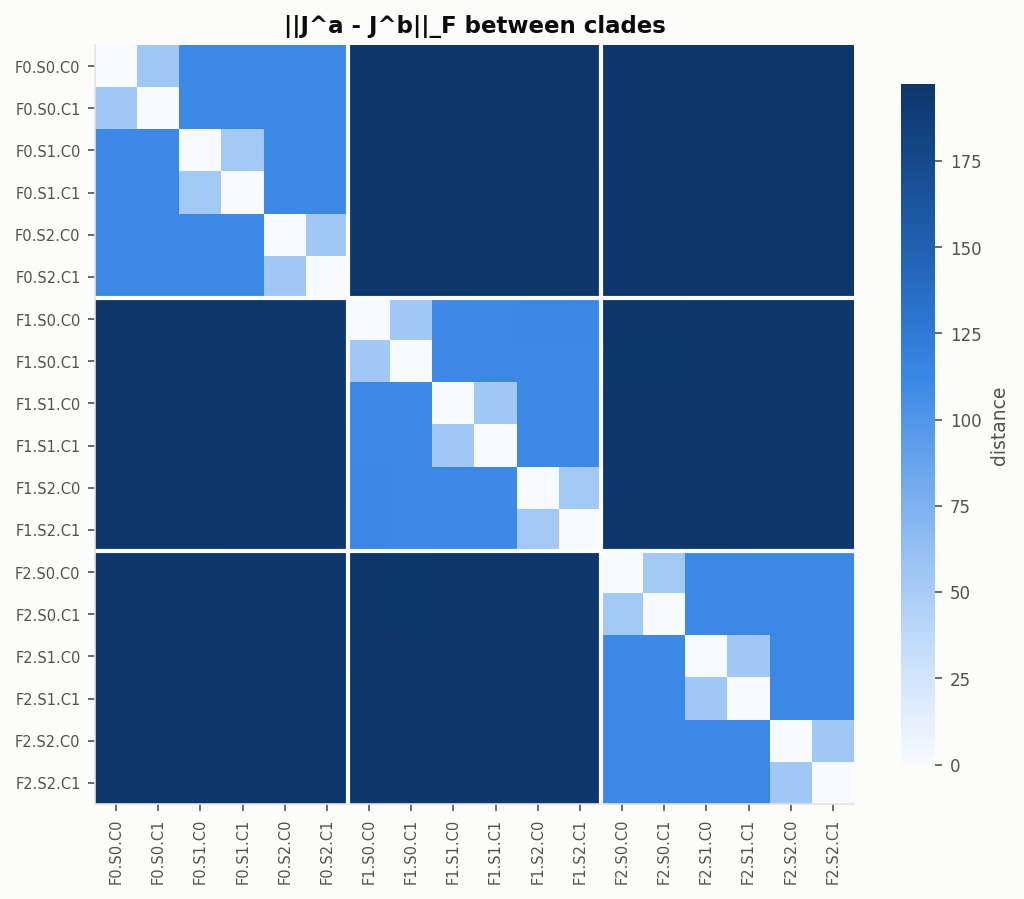
\includegraphics[width=0.49\columnwidth]{ground_truth/01_hierarchy/J_distance_matrix.png}\hfill
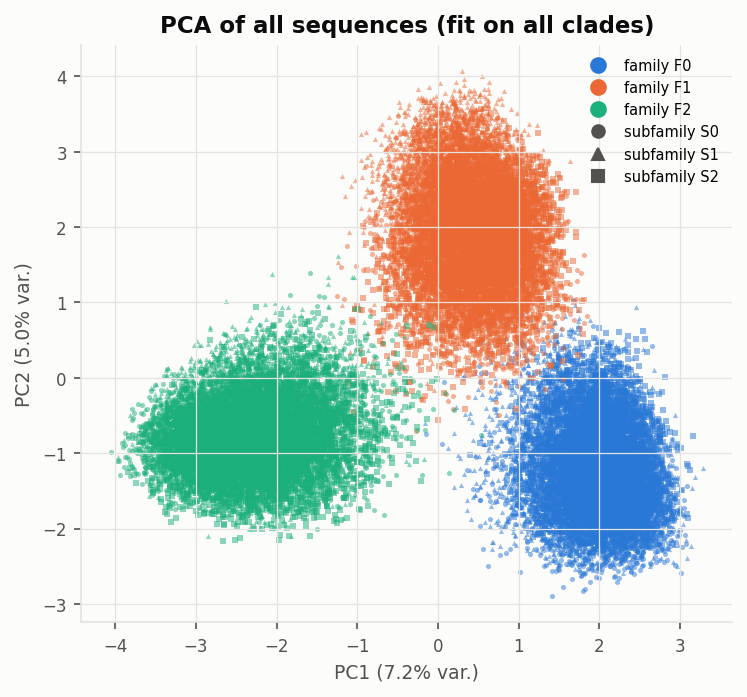
\includegraphics[width=0.49\columnwidth]{ground_truth/03_analysis/pca_all_PC1_PC2.png}
\caption{Left: coupling distances between the 18 clades; the nested blocks are the tree. Right: all sequences on
the first two principal components, coloured by family.}
\label{fig:gt}
\end{figure}

\paragraph{Evaluation.} Generated sets are compared with held-out test sequences through:
\begin{itemize}
\item site frequencies ($r_f$) and connected pair correlations ($r_C$, and the slope of generated vs true $C$);
\item family and clade proportions; each sequence is assigned to the true clade model under which it has the
highest pseudo-log-likelihood (91.5\% correct on labelled clades, 100\% on families);
\item distances: Hamming distance to the nearest training sequence (memorisation), pairwise-distance distributions,
and the Fréchet distance between Gaussians fitted in a fixed 10-dimensional PCA space;
\item where available, the model's conditionals $P(s_i\mid\bm s_{-i})$ on test sequences, compared with the true
clade model's (mean total variation).
\end{itemize}
Fresh samples of the true models (the ``oracle'') give the best achievable score of each metric at the same sample
size.

%=====================================================================
\section{Models}
%=====================================================================
\subsection{Factored attention (a Potts model by construction)}
The couplings are written as attention over positions,
\begin{gather*}
J_{ij}(a,b)=\mathrm{sym}\Big(\sum_{h=1}^HA^h_{ij}V^h(a,b)\Big),\\
A^h=\mathrm{softmax}_j\!\Big(\frac{Q^hK^{h\top}}{\sqrt d}\Big),
\end{gather*}
with positional queries and keys, no self-attention ($A^h_{ii}=0$), and symmetrisation so that the exported $(h,J)$
is a genuine Potts model. Training minimises the pseudo-likelihood
$-\sum_i\log P(s_i\mid\bm s_{-i})$ with an L2 prior. Each block $J_{ij}$ lies in the span of the $H$ value matrices,
and our 179 contact blocks are independent, so exact recovery needs $H\ge179$. We train $H=128$ and $H=256$.

\paragraph{Conditioned version.} Each sequence carries hierarchical tags (family, subfamily, clade). Fields and value
matrices receive additive tag-specific terms, $h(\bm c)=h+\Delta h_f+\Delta h_s+\Delta h_c$ and likewise for $V^h$,
while the attention $A^h$ (which pairs interact) is shared. Tags are dropped hierarchically during training, so that
the model can be conditioned at any level or not at all.

\subsection{Masked diffusion}
Each site is replaced by a mask token with probability $t$ (linear schedule $\alpha_t=1-t$). A bidirectional
transformer (6 layers, width 256, 4.8\,M parameters) receives the partially masked sequence and $t$, and outputs, for
every masked site, a distribution over the 20 residues. It is trained on the MDLM negative ELBO,
\begin{align*}
\mathcal L&=\E_{t\sim U(0,1)}\Big[\frac1t\sum_{i\ \text{masked}}-\log p_\theta(s_i\mid\bm x_t)\Big]\\
&\ge\ -\log p_\theta(\bm s),
\end{align*}
an upper bound on the \emph{full} negative log-likelihood. Training used AdamW, mixed precision and an EMA of the
weights, for 150 epochs (4\,h on one consumer GPU). Generation reveals sites one at a time in random order (the exact
continuous-time limit of ancestral sampling, $L$ network calls per sequence). The model is unconditioned: it never
sees a label.

%=====================================================================
\section{Results}
%=====================================================================
\subsection{Unconditioned factored attention: right contacts, ancestral couplings, wrong family weights}
With $H=128$ the model finds every long-range contact (precision 1.00 when pairs are ranked by $\|J_{ij}\|$ with APC),
even though $H<179$. Comparing the learned $J$ with every node of the tree, the best match is the \emph{average} of the
clades ($r_J=0.69$), then the root (0.65); similarity decreases monotonically towards families, subfamilies and
clades (0.59--0.62). A model trained on the mixture learns what all clades share. All couplings are shrunk (slope 0.57),
and generated correlations are 20--35\% too weak.

\begin{table}[t]
\centering\small
\begin{tabular}{lcccc}
\toprule
family & $\langle E\rangle_F$ & energy & entropy & $\ln\frac{P(F)}{P(\mathrm{F2})}$\\
\midrule
F0 & $-176.1$ & $-10.7$ & $+9.6$ & $-1.12$\\
F1 & $-173.1$ & $-13.7$ & $+12.1$ & $-1.60$\\
F2 & $-186.8$ & 0 & 0 & 0\\
\bottomrule
\end{tabular}
\caption{Why the unconditioned Potts model over-generates family F2. The log-ratio of family weights in the learned
model splits into an energy term and an entropy term (relative to F2), which almost cancel.}
\label{tab:ee}
\end{table}

The striking failure is global: samples are 22/12/66\% from the three families instead of 33/33/33\%. Running
Gibbs chains started inside each family shows this is a property of the learned distribution, not of the sampler.
Writing $\ln P(F)/P(F')=-(\langle E\rangle_F-\langle E\rangle_{F'})+(S_F-S_{F'})$ (Table~\ref{tab:ee}): the most
conserved family F2 has 11--14 units lower energy, a factor $e^{11}$, which its smaller entropy almost cancels.
Equal weights would require the two terms to cancel to $\approx0.1$ nat. That balance is a property of the partition
function $Z$, which pseudo-likelihood never evaluates. Nothing in the loss enforces it.

\subsection{Hierarchical tags fix the proportions; fields carry the fine labels}
The tag-conditioned model ($H=128$) generates the requested clade for 18/18 clade tags, the requested family for
98--99\% of family-tag samples, and the right family proportions when tags are pooled. Per clade $r_C=0.76$, between
the sibling-clade level (0.63) and the oracle (0.83) of Table~\ref{tab:gt}. In PCA-space Fréchet distance, a
generated clade is about 4 times closer to its own clade than the sibling clade is (0.39 vs 1.48), but 20 times
farther than fresh true samples (0.02).

Comparing the learned label-specific changes with the true parent-to-child changes shows \emph{where} the labels are
encoded. For couplings, $r(\Delta J)=0.34,\ 0.21,\ 0.11$ at family, subfamily and clade level. For fields,
$r(\Delta h)=0.58,\ 0.50,\ 0.33$, about twice as high at every level. The couplings resolve the family; the
subfamily and clade are carried mainly by the fields. Without a tag, the conditioned model's family weights are again
wrong (33/21/46\%): the same pseudo-likelihood blind spot.

\paragraph{More heads.} With $H=256$ couplings are recovered better (unconditioned: $r_J$ 0.69$\to$0.77, slope
0.57$\to$0.62), as the rank argument predicts. Samples do not improve: the unconditioned family weights get worse
(11/13/76\%), and the conditioned model's doubled label tables over-fit before the fields are learned. The best Potts
generator remains the conditioned $H=128$ model.

\subsection{Masked diffusion: right proportions without labels}
\begin{figure*}[t]
\centering
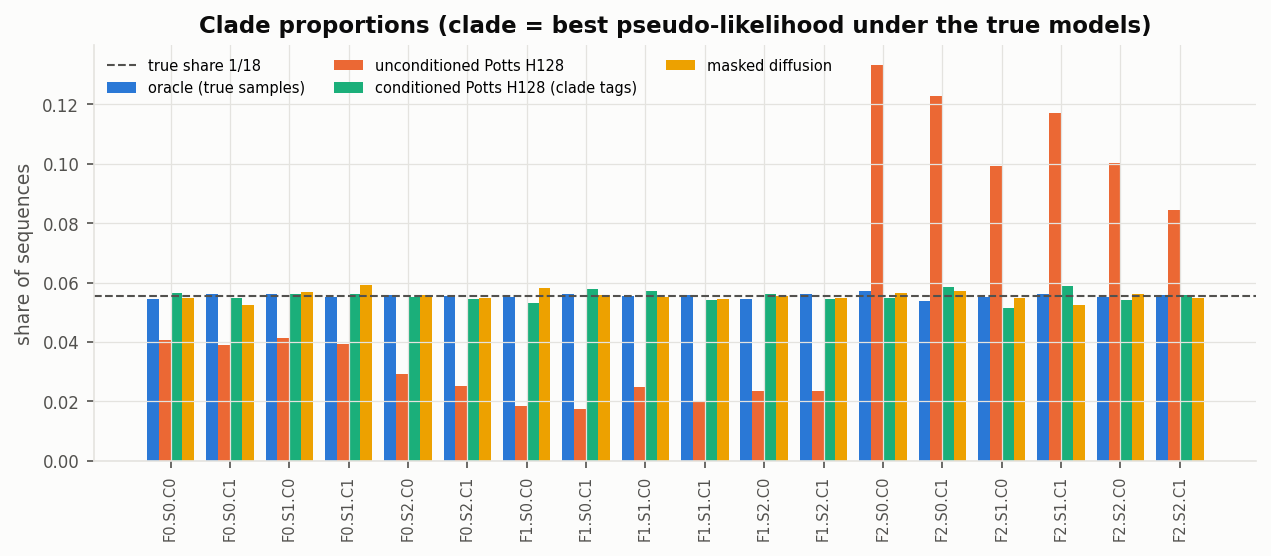
\includegraphics[width=0.85\textwidth]{comparison/clade_proportions.png}
\caption{Share of generated sequences assigned to each of the 18 clades. Dashed: the true share 1/18. The
unconditioned Potts model concentrates on family F2; the diffusion model, without labels, is uniform.}
\label{fig:props}
\end{figure*}

The diffusion model generates the families in proportions 33.4/33.4/33.2\% and the 18 clades within total variation
0.011 of uniform (fresh true samples: 0.005), without ever seeing a label
(Fig.~\ref{fig:props}). Its pooled statistics are practically those of true samples (Table~\ref{tab:all}): $r_C=0.992$
against 0.994, Fréchet distance 0.005 against 0.001. Per clade, it matches or beats the Potts model that is
\emph{given} the clade tag ($r_C$ 0.764 vs 0.751, Fréchet 0.14 vs 0.33). It does not memorise: no generated sequence is
a training sequence, and the nearest-neighbour distance to the training set (0.393) is close to that of held-out true
sequences (0.378).

\begin{table*}[t]
\centering\small
\begin{tabular}{lccccccc}
\toprule
 & uses & family shares & clade TV & pooled & per-clade & per-clade & conditionals:\\
 & labels & F0/F1/F2 (\%) & to uniform & $r_C$ & $r_C$ & Fréchet & TV to truth\\
\midrule
oracle (fresh true samples) & -- & 33/33/33 & 0.005 & 0.994 & 0.828 & 0.032 & 0\\
unconditioned Potts, $H=128$ & no & 22/13/66 & 0.324 & 0.895 & 0.562 & 1.716 & 0.154\\
unconditioned Potts, $H=256$ & no & 11/14/76 & 0.424 & 0.855 & 0.555 & 1.448 & 0.152\\
conditioned Potts, $H=128$ & tags & 33/33/33 & 0.013 & -- & 0.751 & 0.332 & 0.100\\
\textbf{masked diffusion} & \textbf{no} & \textbf{33/33/33} & \textbf{0.011} & \textbf{0.992} & \textbf{0.764} & \textbf{0.136} & 0.102\\
\bottomrule
\end{tabular}
\caption{All models on the same footing. Generated sequences are assigned to clades by the true-model
pseudo-likelihood classifier; per-clade metrics compare the sequences assigned to clade $c$ with the test sequences
of $c$. Last column: mean total variation between the model's $P(s_i\mid\bm s_{-i})$ and the true clade model's, on test
sequences (the conditioned Potts model is given the true tag).}
\label{tab:all}
\end{table*}

\paragraph{The probabilities themselves.} Masking one site of a test sequence and reading the network's output gives
its conditional $P_\theta(s_i\mid\bm s_{-i})$. These are as close to the true clade conditionals (mean TV 0.102) as
those of the conditioned Potts model given the true tag (0.100), and much closer than the unconditioned Potts
model's (0.154). The network infers the clade from the other 59 residues.

\paragraph{The sampler matters.} With few reverse steps, several sites are revealed at once and drawn independently.
Correlations then weaken: the slope of generated vs true correlations is 0.81 with 15 steps, 0.94 with 60, 0.98
with 240, and 0.985 for the exact one-site-at-a-time sampler, which costs the same as 60 steps.

\paragraph{Remaining defects.} Within-family correlations are still about 10\% too weak (slope 0.89). Training had not
fully converged (the best epoch was the last, though the last 100 epochs gained only 0.025 nats per site). The
denoiser essentially ignores its time input, as the theory predicts for the optimal denoiser of masked diffusion.

%=====================================================================
\section{Discussion}
%=====================================================================
\paragraph{What pseudo-likelihood cannot learn.} The pseudo-likelihood fits each conditional $P(s_i\mid\bm s_{-i})$,
and these are blind to how much total probability each region of sequence space receives. For a multi-family
distribution, the relative family weights are a global quantity, set by a near-cancellation between energy and
entropy that only the partition function sees. Every Potts model we trained by pseudo-likelihood without tags got them
wrong, and more capacity made it worse. Tags remove the problem by construction. A likelihood-based objective, here
the diffusion ELBO, removes it without labels.

\paragraph{What a Potts model learned from a mixture represents.} Trained on pooled clades, the Potts model's couplings
are closest to the ancestral and average models, and shrunk. A single Potts model cannot represent a mixture exactly,
and part of its coupling budget goes into approximating the mixture structure rather than the within-clade
interactions. When tags are available, the label-specific information lands mostly in the fields. Inferring
clade-specific couplings would need either more data per clade or a stronger structural prior.

\paragraph{Interpretability versus fidelity.} The factored-attention model is a Potts model: its contacts and
couplings can be read off and compared with the truth, and it is small (0.5--2\,M parameters) and fast to train
(2--23 minutes). The diffusion model is the better generator and gives correct conditional probabilities without
labels. But it is 2--9$\times$ larger, 10--100$\times$ more expensive to train, and offers no explicit coupling
tensor.

\paragraph{Limitations.} The benchmark is synthetic: contact blocks are drawn independently (the hardest case for
low-rank couplings, unlike real proteins), all clades share one fold, and there are no insertions or deletions. Each
configuration was trained once (one seed). The clade assignment used to compute per-clade metrics is itself 91.5\%
accurate.

%=====================================================================
\section{Conclusion}
%=====================================================================
On a controlled hierarchical benchmark, a Potts model learned by factored attention and pseudo-likelihood recovers the
contacts and the shared, ancestral part of the couplings. It cannot get the global family weights right without
labels, a direct consequence of never seeing the partition function. Hierarchical tags fix the weights, and the
fine-grained labels are then carried by the fields. A masked diffusion model trained on a likelihood bound reproduces
the family and clade structure without labels, at the level of the tag-conditioned Potts model or better, at the cost
of interpretability and training time.

We have also started to study \emph{how} the diffusion model generates: when a trajectory commits to its family,
subfamily and clade (speciation), and when the exact optimum of its loss would collapse onto a training sequence
(memorisation). This follows Biroli, Bonnaire, de Bortoli and Mézard (\emph{Nat.\ Commun.} 2024), transposed from
Gaussian noise to masking. Initial results, a top-down cascade of commitments and a collapse time predicted by a
parameter-free theory, are reported in Part~IV of \texttt{docs/modelization.pdf} and in the notes in
\texttt{docs/notes/}.

\paragraph{Code and data.} Code, configurations, data splits, trained models and the full document are available at
\url{https://github.com/yk985/hierarchical-_Potts_models_learning}.

\end{document}
